\chapter{System Implementation}\label{cha:Implementation}
In this chapter, we will talk about the implementation datail of the proposed system and will focus on the function on data service server's environment and techeniques.

\section{Data Service Server Environment}

\subsection{Node.js}
Node.js \cite{nodejs} is a open sourse JavaScript application framework written in C \cite{clang}, C++ \cite{cplus} and JavaScript \cite{javascript}
Node.js can run on many operation systems like Microsoft Windows, Linux, Mac and embedded system like Raspberry, Cubieboard.
There are many advantages of Node.js.
To begin with, it use V8 JavaScript engine to boost performance, which make it much more better than other script language.
Second, it's event driven and non-blocking I/O feature is surprisingly appropriate to both front-end and back-end of web application.
Third, as a popular programming language like Python and Ruby, there are many third-party module on the word wild web that developers around the world wrote,
we can make use of these modules to accelerate time developing apps. Whats more, the module is managed properly by nodejs package management (npm), which make it easy to import modules.
\subsection{Asynchronous Process Control}
Since Node.js is JaveScript with extensional function, the event-driven feature in JaveScript is to Node.js, as a result we can often see asynchronous design model in JavaScript code.
The idea of event-driven and asynchronous is run the job need long time to finish in the back-end event engine to avoid the job block all the process.
After that, we will set a callback function to inform the process when the time-comsuming job is done.
Figure \ref{fig:asynchornous} shows the idea of asynchronous process control.

\begin{figure}[H]
    \centering
    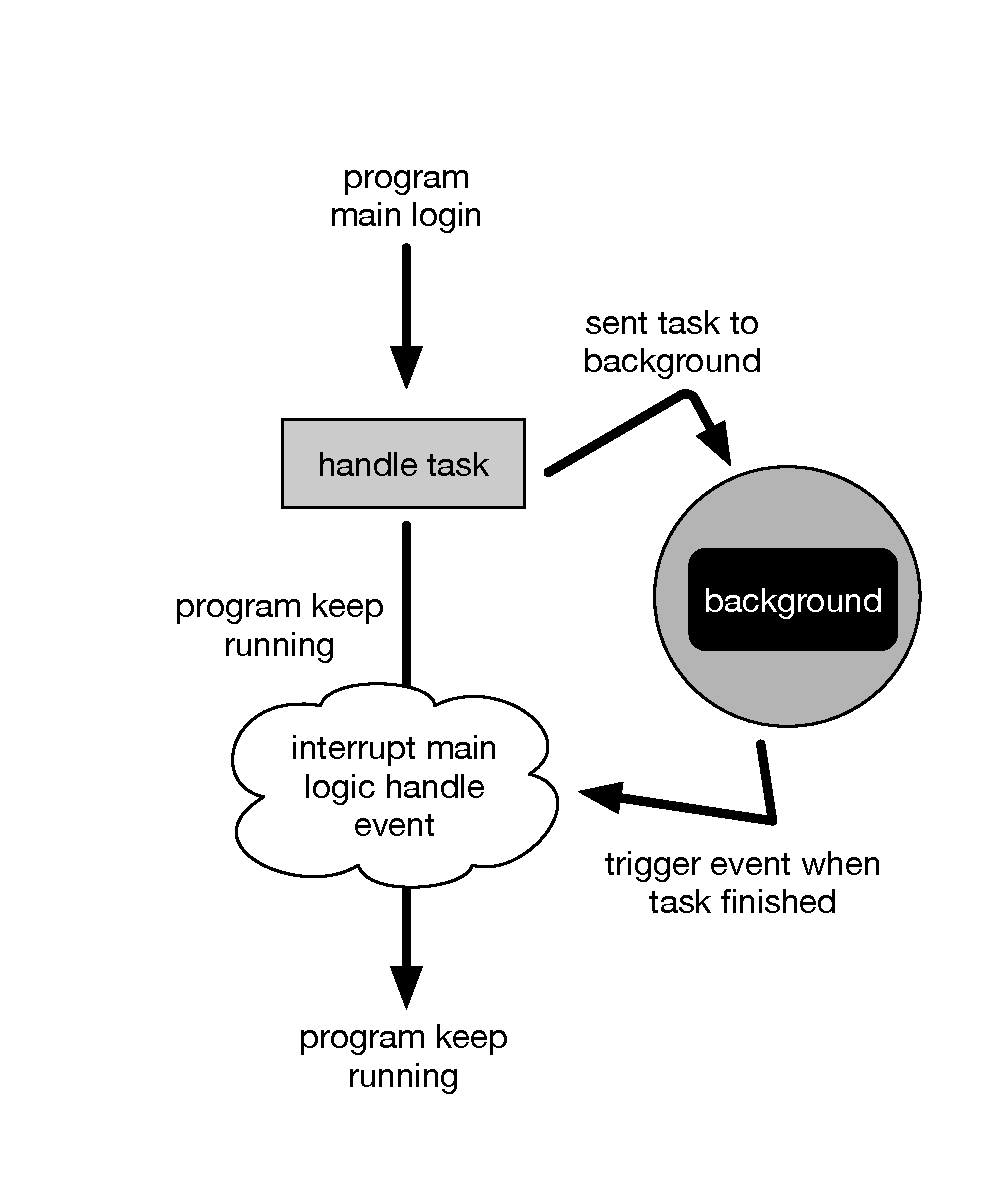
\includegraphics[width = 0.8\textwidth]{fig/asynchonous-process.eps}
    \caption{Asynchorous process control model}
    \label{fig:asynchornous}
\end{figure}


\subsection{MongoDB}
MongoDB \cite{mongodb} is an free and open source nosql database, data in mongodb saved as a json-like document with dynamic schemas (BSON).
MongoDB can handle big data in scale in Terabytes with its high performance and it's tableless database structure also make it easy to integrate data in certain type of applications eaiser and faster.

\subsection{Google Cloud Platform}
Google Cloud Platform \cite{googlecloud} is a platform integrates Iaas, Paas and Saas.
According to the website, it provides eight categories of service, including basic virtual machine renting, database hosting, big data analysis, machine learning and more.

\subsection{Iron Worker}
Ironworker \cite{ironworker} is a service on Iron.io, which make developer setup a worker on website with flexible scheduling setting.
Once developer setup the worker, Ironworker will monitor the worker, and if any thing go wrong, Ironworker will notify you by email with detail information.

\subsection{Jieba}
Jieba \cite{jieba} is a open source python chinese text secmentation module which provide friendly API for developers, it is now support python2, python3 and can be installed by pip or other python package management module.
Jieba segment the text by it's own dictionary on default, however it allow developers to edit or replace the dictionary which Jieba used to segment text.
In our analysis system, we use this flexible tool to segment out subtitle base on our custom dictionary file.

\section{Server Setup}
In order to construct out server, we rent a VM instance machine type:n1-standard-4 (4 vCPUs, 15 GB memory), and on top of that we run a mongoDB on the same machine.
After setting up the environment, we execute the nodejs api server conneted with the mongoDB to save the data to database and to provide other API for query data.
Among APIs the server provide, there is a API will triggered by the worker we set onece a day, this API is designed for execute a python script, which is our data analysis system that will update the refine data (see Figure \ref{fig:serversetup}).
\begin{figure}[H]
    \centering
    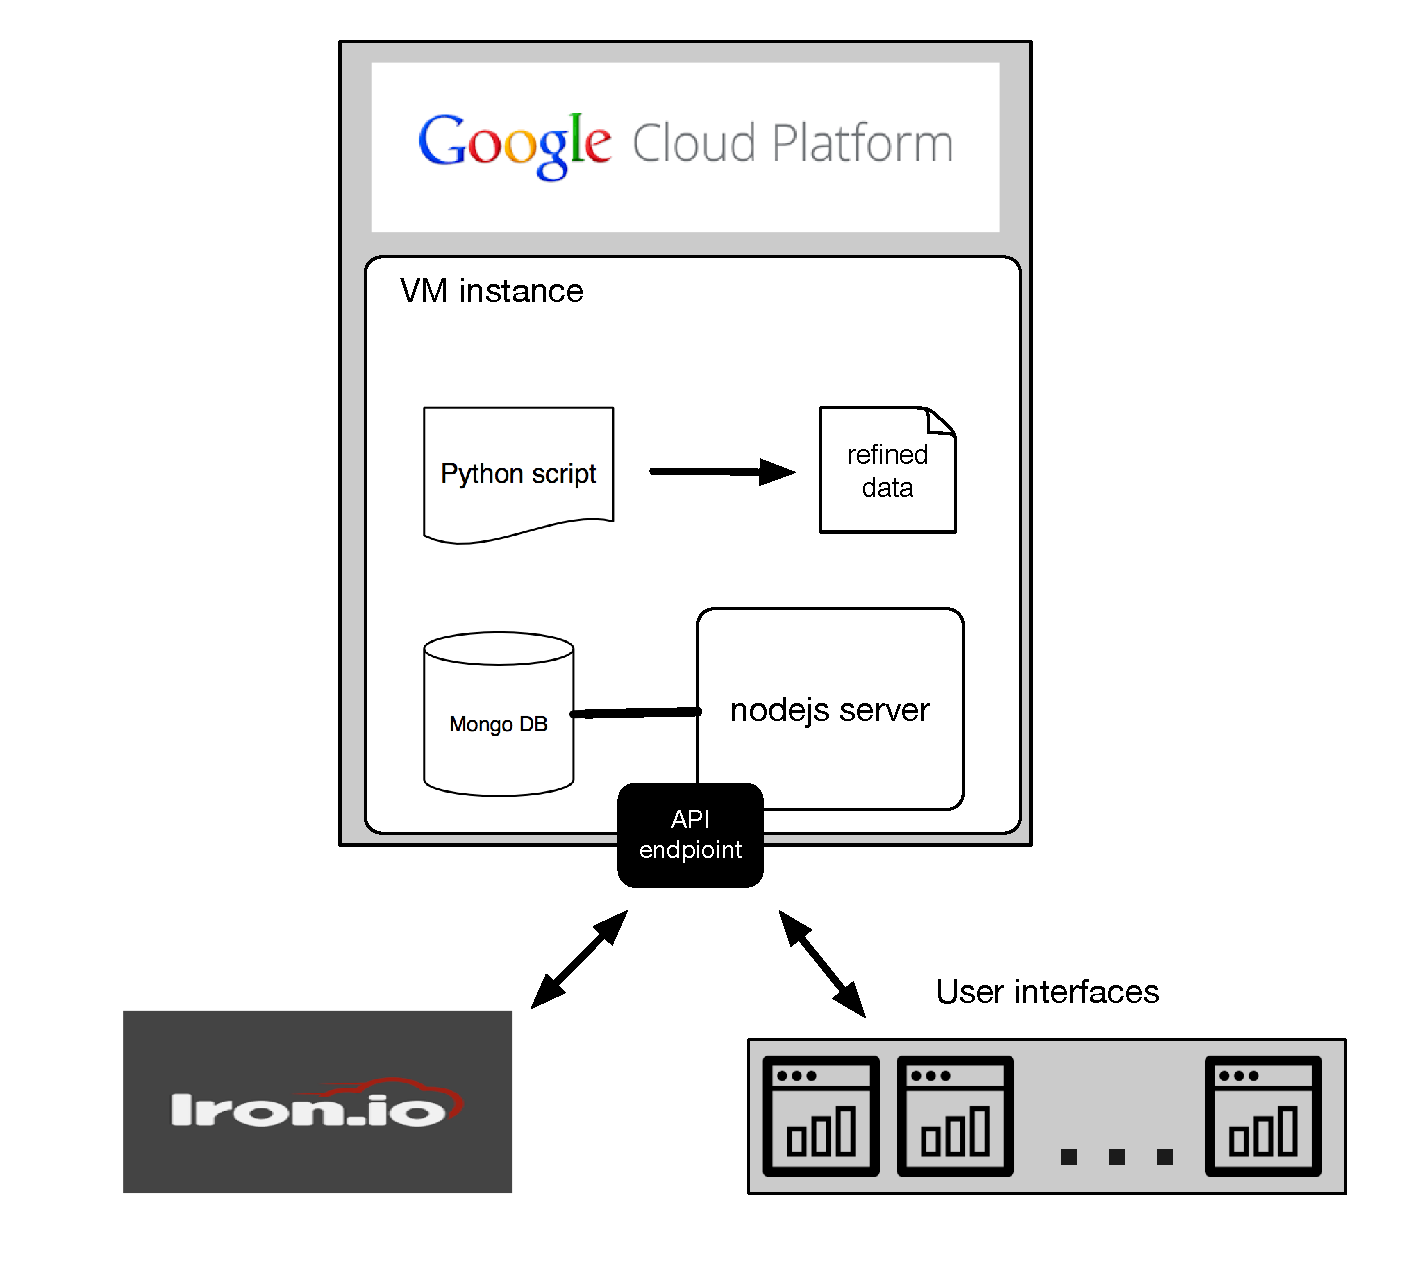
\includegraphics[width = 0.8\textwidth]{fig/serversetup.eps}
    \caption{server setup}
    \label{fig:serversetup}
\end{figure}

\section{Data Service API}
\subsection{API's Collects User Activity Records}
We discussed activity models in Chapter \ref{cha:architecture}, in table \ref{table:collectact} shows the APIs that data service server provided for recording activity records belong to different activity models, and the schema column of table pictures out the data structure stored in mongoDB.
Among the sehema of all model, action field denote the situation user interacted with the platform object.

\begin{table}[H]
\centering
\begin{tabular}{|l|l|l|l|}
\hline
method & url            & purpose                              & schema                                                                                                                                                                                                                                                                                                                     \\ \hline
POST   & /login\_data   & records user's log in/out activity   & \begin{tabular}[c]{@{}l@{}}action: String\\ userId: Number\\ userAccount: String\\ time: ISODate\end{tabular}                                                                                                                                                                                                              \\ \hline
POST   & /page\_data    & records user's trail on website      & \begin{tabular}[c]{@{}l@{}}action: String\\ userId: Number\\ userAccount: String\\ page: String\\ courseId: Number\\ chapterId: Number\\ time: ISODate\end{tabular}                                                                                                                                                        \\ \hline
POST   & /article\_data & records user's forum activity        & \begin{tabular}[c]{@{}l@{}}action: String\\ userName: String\\ userId: Number\\ userAccount: String\\ courseId: Number\\ object\_article\_info:\\ \{\\ article\_id:Number\\ article\_author\_id:Number\\ article\_type:String\\ aritcle\_course\_id:Number\\ article\_chapter\_id:Number\\ \}\\ time: ISODate\end{tabular} \\ \hline
POST   & /post\_data    & records user's exercise activity     & \begin{tabular}[c]{@{}l@{}}exerciseId: Number\\ exerciseType: String\\ correctAns: String\\ execOrder: Number\\ courseId: Number\\ getScore: Boolean\\ execTotalCount: String\\ userId: Number\\ studentAns: Array\\ time: ISODate\end{tabular}                                                                            \\ \hline
POST   & /video\_data   & records user's video player activity & \begin{tabular}[c]{@{}l@{}}action: String\\ userId: Number\\ userAccount: String\\ videoStartTime: Number\\ videoEndTime: Number\\ videoId: Number\\ videoTotalTime: Number\\ courseId: Number\\ chapterId: Number\\ chapterVideoCount: Number\\ chapterVideoOrder: Number\\ playRate: Number\\ time: ISODate\end{tabular} \\ \hline
\end{tabular}
\caption{APIs records user activity}
\label{table:collectact}
\end{table}

\section{Analysis System}
Anaylysis system is a important role of the proposed system, we use users' video watching activity records to observe users' watching patterns and find out video sections that are possibley is the difficult part in lecture video for users, we call these video sections ``hot segment''.
As long as we find out hot segment, we integrate further these hot segments with video subtitles to map out what concepts were mentioned in the video section, which is ``Videomark'' in this thesis.
In this section we will explain how we generate Videomark with combination of difficult lecture videos section and semented subtitle.

\subsection{Counting the Video Seek Events}
The collected video seek event refer to the event that leaners drag the play bar to relocate the start point of the video while watching a video. In other words, two specific time stamps, the start time and the end time, are collected. The end time is the starting point of the specific part that leaners want to watch again.
Considering the continuation of the timeline, the timeline is split into small segments to improve the accuracy of the concept for further analysis. In this study, based on the experiments, the duration of a segment is designed to have 40 seconds. Thus, the 1st segment is from 1 to 40 seconds, the 2nd segment is from 41 to 80 seconds, and son on.
Nevertheless, a learner usually didn’t drag the play bar to the correct watching position at the first time. It is found that the average number of seeking events before the learner getting the final position is around 2 to 5. These kinds of seeking events should be ignored as they are just for “looking” the right position. To do this, a seek event is ignored if the time interval between this seek event with its previous seek event is less than two seconds.
To find out the ``hot learning interests or difficult point'', the``hot segment'' of the video are first identified based on the number of video seeking events and then the ``keywords'' included in the subtitles of these hot segments were processed, see Figure \ref{fig:countseek}.

\begin{figure}[H]
    \centering
    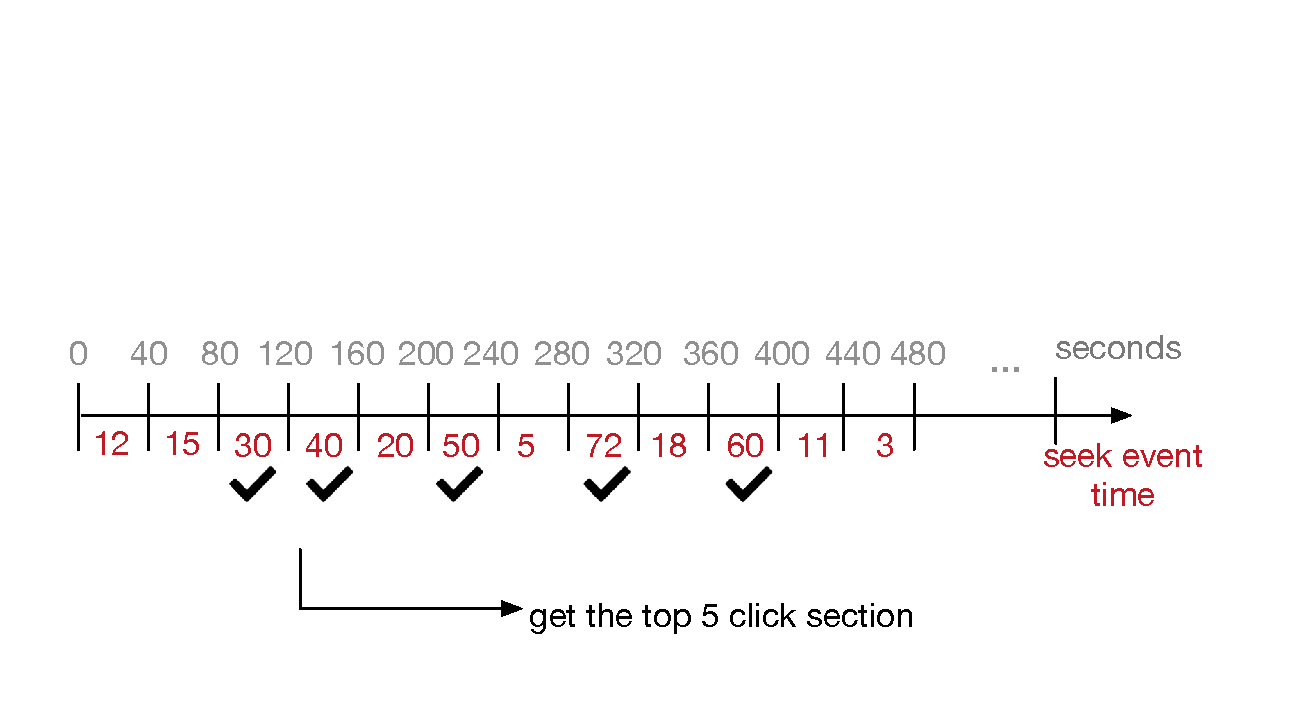
\includegraphics[width = 0.8\textwidth]{fig/countseek.eps}
    \caption{counting seek event find hot sections}
    \label{fig:countseek}
\end{figure}

\subsection{Subtitle Segmentation}
The subtitles of the videos are processing to extract the ``keyword'' of the learning concept. In this thesis, all the subtitles are provided by Chinese. Jieba is used to split subtitles into several meaningful chunks of word in the sentence level.
To improve the accuracy, two extra processing were used. First of all, since the contents of subtitles are colloquial, some stop-words will be mistakenly seen as keywords, such as ``this'', ``that'', ``because'', and ``so''. Therefore, those stop words are added into the stop-word dictionary to avoid the redundancy. Secondly, the word-frequency dictionary is adjusted for better Jieba results. The keyword-frequency stands for the keyword weight. The higher the weight of a keyword, the more likely the keyword is valued as a meaningful chunk.
Finally, if some teacher wants to make keyword more precisely we will ask them provide a concept file, this concept file will act as a fileter leave only words in file, Figure \ref{fig:subtitleseg} illustrate the idea of subtitle segmentation.
The results of processed subtitles (keywords) are combined with the seek event counts (hot segments) to identify the “hot keywords” of the specific topic.

\begin{figure}[H]
    \centering
    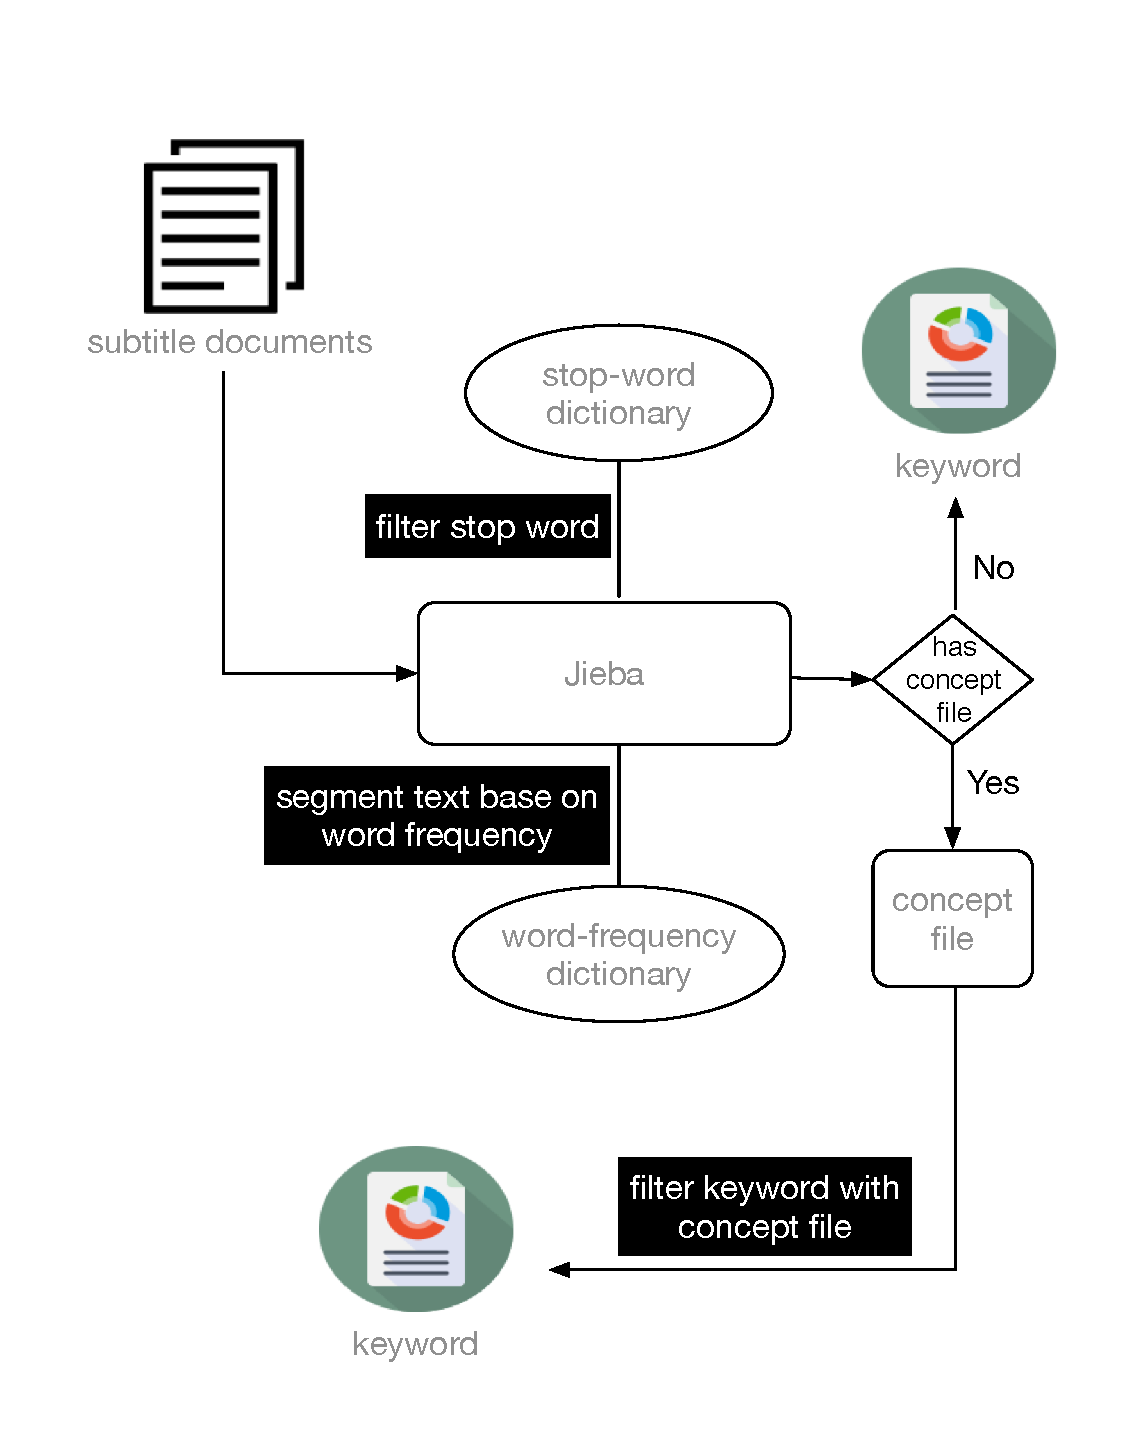
\includegraphics[width = 0.8\textwidth]{fig/subtitleseg.eps}
    \caption{subtitle segmentation}
    \label{fig:subtitleseg}
\end{figure}

\subsection{Weighting the Keyword}
After the preprocessing of the video seek event counts and identified keywords, the third step is to calculate the weight of each of the keywords. In this study, for each video, the top five weighted keywords are collected into the keyword cloud.
Figure \ref{fig:keywordcloud} depicts the “keywords cloud” of week 1 of the course 2016 spring Network Security on ShareCourse. The larger size of keyword means that more learners are interested or feel difficulty in that keyword (concept). Thus, the video segments introducing this keyword were watched more frequently.
For example, in Figure \ref{fig:keywordcloud}, the ``SYN'', ``DDoS'' and ``Flooding'' are the biggest (hottest) three keywords in the keywords cloud, meaning that those concepts are most interested in or difficult of the learners.

\begin{figure}[H]
    \centering
    \includegraphics[width = 0.8\textwidth]{fig/wordcloud.png}
    \caption{keyword cloud example}
    \label{fig:keywordcloud}
\end{figure}

\section{User Interface}
\subsection{Environment}
\subsubsection{ShareCourse}
ShareCourse \cite{sharecourse} is a famous MOOCs platform in Chinesspeaking countries, which provides both Web and mobile service.
Since 2012, ShareCourse has been providing more than 1,000 courses with over 60 cooperative universities in Taiwan.
Up to the precent, more than 60000 students have registered on ShareCourse.
ShareCourse provide a environment with complete functions for MOOCs learners in terms of instructional videos, peer-grading quiz/assignment, discussion forum, weekly exercise, and certificate.

\subsubsection{D3-cloud.js}
D3-cloud \cite{d3cloud} is a JavasCript module which can make texts turn into cloud layout on the web page, we use d3-cloud to present the result of data analysis system to user, providing them a friendlier and fancier data visualization view.

\subsubsection{Boostrap}
Bootstrap\cite{bootstrap} is a open-source and free front-end web framework for design website and web applications, it contains html, css and javascirpt-based template for typography.
Useful elements such as buttom, modal, grid system and more are provided which makes developers create beautiful custom website easily.

\subsubsection{jQuery}
jQuery is a \cite{jquery} cross browser javascript library simplify the manipulation of javascript to controll html DOM elements and provides features like event-handle, animation and ajax.
Ajax, one of the feature of jQuery, make it possible to perform cross-browser Ajax requests using \code{\$.ajax}, Figure \ref{fig:ajaxpost} sohws an code that ajax post a hash variable \code{data} to url \url{http://API_endpoint/saveData}.
If the request successd \code{.done()} in line 8 will be triggered; otherwise \code{.fail()} in line 10 will be triggered.
This kind of usage in example can be linked with elements in web page to create different user interactive scenarios.
Ajax also follows the asynchornous mechanism so that any single ajax execution or failure will not cause page crash or been locked.

\begin{figure}[H]
    \centering
    \includegraphics[width = 0.9\textwidth]{fig/ajax-example.png}
    \caption{Ajax post example}
    \label{fig:ajaxpost}
\end{figure}

\subsection{Video Mark Page}
All the video mark feature are start with the keyword cloud, we add a button at bottom of lecture video page labled with ``keyword cloud'' as shown in Figure \ref{fig:cloudbutton}.

\begin{figure}[H]
    \centering
    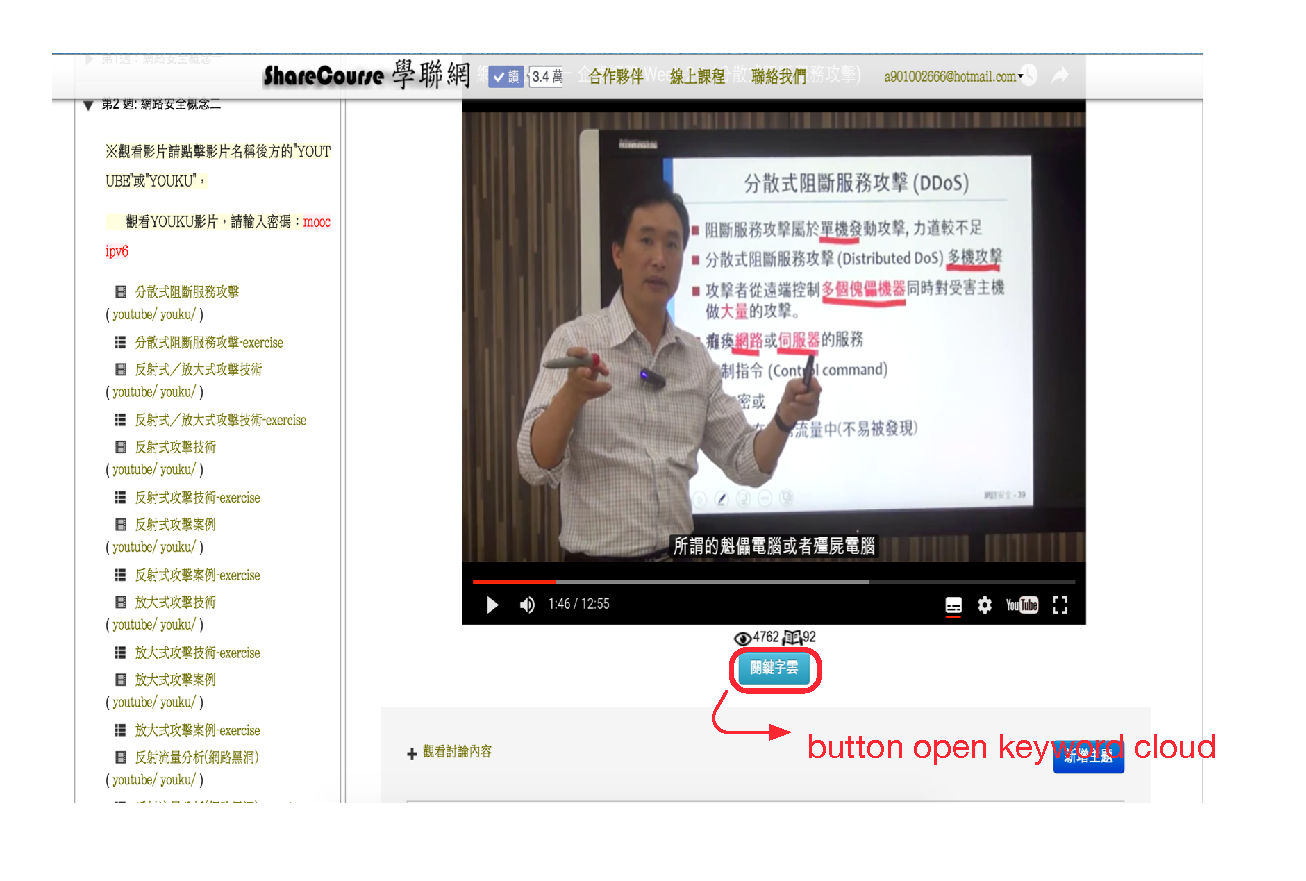
\includegraphics[width = 0.9\textwidth]{fig/cloudbutton.eps}
    \caption{video mark feature open keyword cloud button}
    \label{fig:cloudbutton}
\end{figure}

Once the button been clicked, the brwoser will use ajax to send a post request to data service server to get weighted keyword datas.
The return data of ajax request will be a json fomat containing keywords in the chapter that user is now watching at, moreover, each keyword will connect to a bounch of concept-related video information.
D3-cloud.js will handle the json data afterward and draw out the keyword cloud see Figure \ref{fig:cloudopened}.

\begin{figure}[H]
    \centering
    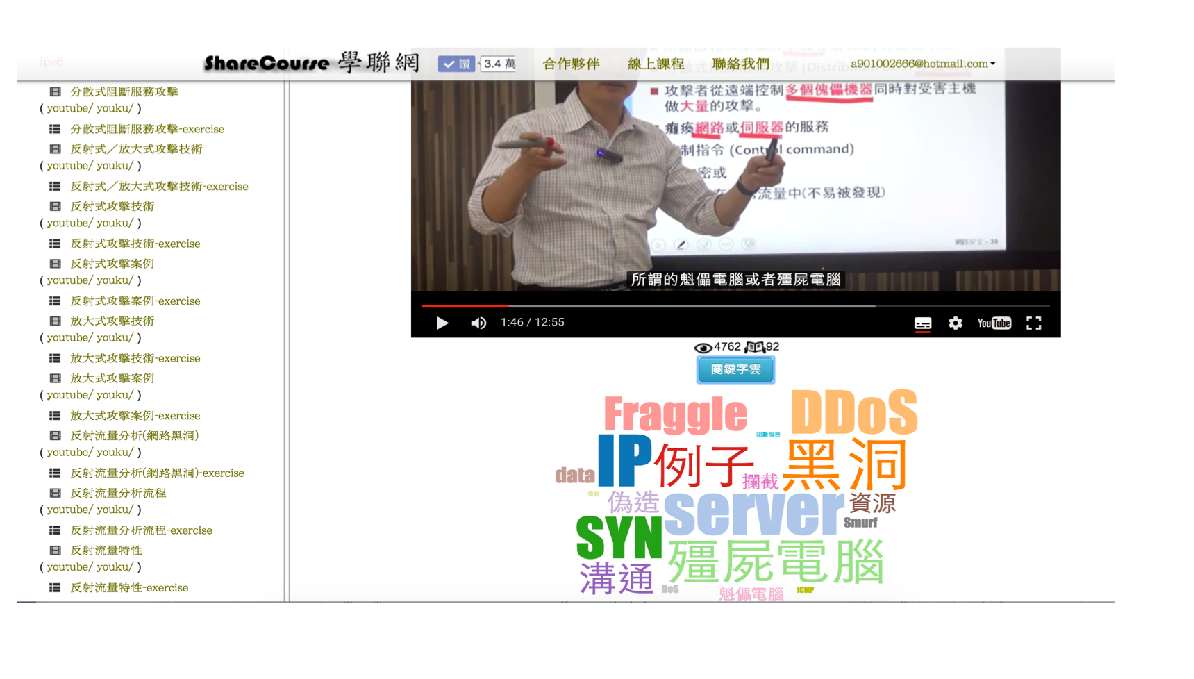
\includegraphics[width = 0.8\textwidth]{fig/cloudopened.eps}
    \caption{keyword cloud shows up}
    \label{fig:cloudopened}
\end{figure}

In keyword cloud, size of keyword reveal how important the keyword is, and the information of keyword size will be in the return data of API we mentioned above.
In fact, keywords in keyword cloud will be a clickable button, and if the keyword is clicked, another section contains multiple hyperlink, we call it hypelink section, will show up at the bottom of keyword cloud.
Figure \ref{fig:keywordurl} shows the result we click ``DDos'' in keyword cloud, and a section contains four hyperlinks shows up.
\begin{figure}[H]
    \centering
    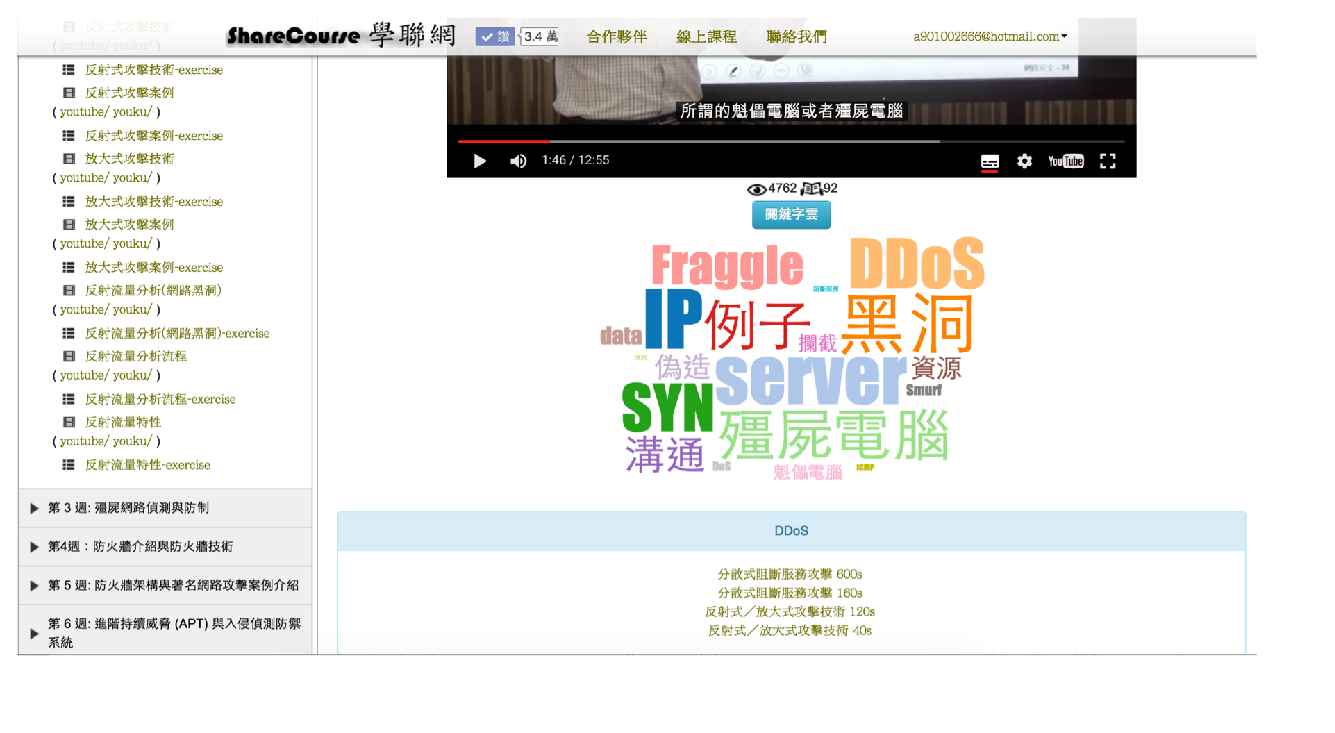
\includegraphics[width = 0.8\textwidth]{fig/keywordurl.eps}
    \caption{hyperlinks show up on click the keyword in cloud}
    \label{fig:keywordurl}
\end{figure}

For each hyperlink, the label is used to tell users the hyperlink will bring them to which video and on which seconds in this chapter.
In Figure \ref{fig:openvideotab} show the result we click the first hyperlink or DDos hyperlink section, a tab of video player poped up and start the video from 10:00(600) seconds which matchs the seconds of hyperlink label and the video is talking about DDos as well.

\begin{figure}[H]
    \centering
    \includegraphics[width = 0.8\textwidth]{fig/openvideotab.eps}
    \caption{open new tab playing start from video mark}
    \label{fig:openvideotab}
\end{figure}
